\documentclass[12pt, a4paper, ngerman]{article}
\title{AD-DA Wandler}
\author{Paul Walker \& Jens Hocke}
\date{29.09.2021}
\newcommand{\Autor}{Paul Walker \& Jens Hocke}
\newcommand{\Kurs}{INF20IN}
\newcommand{\MatrikelNummer}{}
\newcommand{\Was}{Laborbericht}
\newcommand{\Studiengang}{Informatik / Informationstechnik}

% \usepackage{biblatex} % für bibliografie
\usepackage{hyperref} % für links zum klicken
% \usepackage{color}    % für Farben (benötigt für listings)
% \usepackage{listings} % code schnipsel
\usepackage[ngerman]{babel} % lokalisierung der Titel (Inhaltsverzeichniss)
\usepackage{bookmark} % bookmarks für das PDF
\usepackage{csquotes} % korrekte quotes
\usepackage[version=3]{acro} % akronyme
\usepackage{geometry} % seitengeometrie (margin etc einstellen)
\usepackage{parskip}  % zeilenabstand bei neuem paragraph statt indentierung
\usepackage{fancyhdr} % header und footer
% \usepackage{fontawesome5} % icons
% \usepackage{array}    % für bessere Tabellen
\usepackage{titlesec} % um die Titel anzupassen
\usepackage{graphicx} % für graphiken

\graphicspath{{./assets/}}

\hypersetup{
  pdfauthor={\Autor},
  pdftitle={\Was},
  hidelinks
}

\geometry{
  a4paper,
  left=25mm,
  right=25mm,
  headheight=125mm,
  top=35mm,
  bottom=30mm,
  footskip=15mm
}

% title setup 
% make paragraph have a newline
\titleformat{\paragraph}
{\normalfont\normalsize\bfseries}{\theparagraph}{1em}{}
\titlespacing*{\paragraph}
{0pt}{3.25ex plus 1ex minus .2ex}{1.5ex plus .2ex}

% add bibliography (should we need one)
% \addbibresource{bibliography.bib}

% header and footer setup
\pagestyle{fancy}
\fancyhf{}
\rhead{\Was}
\lhead{\leftmark}
\lfoot{Autoren: \Autor, Kurs: \Kurs}
\rfoot{Seite \thepage}
\renewcommand{\headrulewidth}{1pt}
\renewcommand{\footrulewidth}{1pt}
\fancypagestyle{simple}{
  \fancyhf{}
  \rhead{\Was}
  \lfoot{Autor: \Autor, Kurs: \Kurs}
  \rfoot{Seite \thepage}
}

% acronyms
\acsetup{
  list/display = used,
  pages/display = first
}
\DeclareAcronym{adc}{short=ADC, long=Analog Digital Converter}
\DeclareAcronym{dac}{short=DAC, long=Digital Analog Converter}
\DeclareAcronym{inl}{short=INL, long=Integrale Nichtlinearität}
\DeclareAcronym{dnl}{short=DNL, long=Differenzielle Nichtlinearität}
\DeclareAcronym{dmm}{short=DMM, long=Digitales Multimeter}
\DeclareAcronym{ttl}{short=TTL, long=Transistor Transistor Logik}
\DeclareAcronym{led}{short=LED, long=Light Emitting Diode ,first-style=short,subsequent-style=short}

\begin{document}

% Titlepage
\makeatletter
\begin{titlepage}
  \begin{center}
    \vspace*{1cm}
    {\Huge\scshape \Was}\\[2cm]
    \begin{center}
      \linespread{1}\Huge \@title\\[2cm]
    \end{center}
    {\large Studiengang \Studiengang}\\
    {\large an der Dualen Hochschule Baden-Württemberg\\ Stuttgart}\\[2cm]
    {\large von}\\
    {\large\bfseries \@author}
    \vfill
  \end{center}
\end{titlepage}
\makeatother

% Table of content
\tableofcontents

\newpage
\thispagestyle{simple}
\printacronyms[name=Abkürzungsverzeichnis, heading=section*]
\newpage

\section{Versuch Nr.1}

Es soll die \ac{inl} und die \ac{dnl} im mittleren Bereich,
sowie die Konversionsrate des \ac{adc} gemessen werden.

\subsection{Genutze Geräte und Bauteile}

\ac{dmm}: FLUKE 87 V True RMS Multimeter \\
Netzgerät: BASETech BT-153 \\


\subsection{Versuchsaufbau}

\begin{figure}%[h] % das h sorgt dafür dass es genau an der Position im text steht.
  \centering
  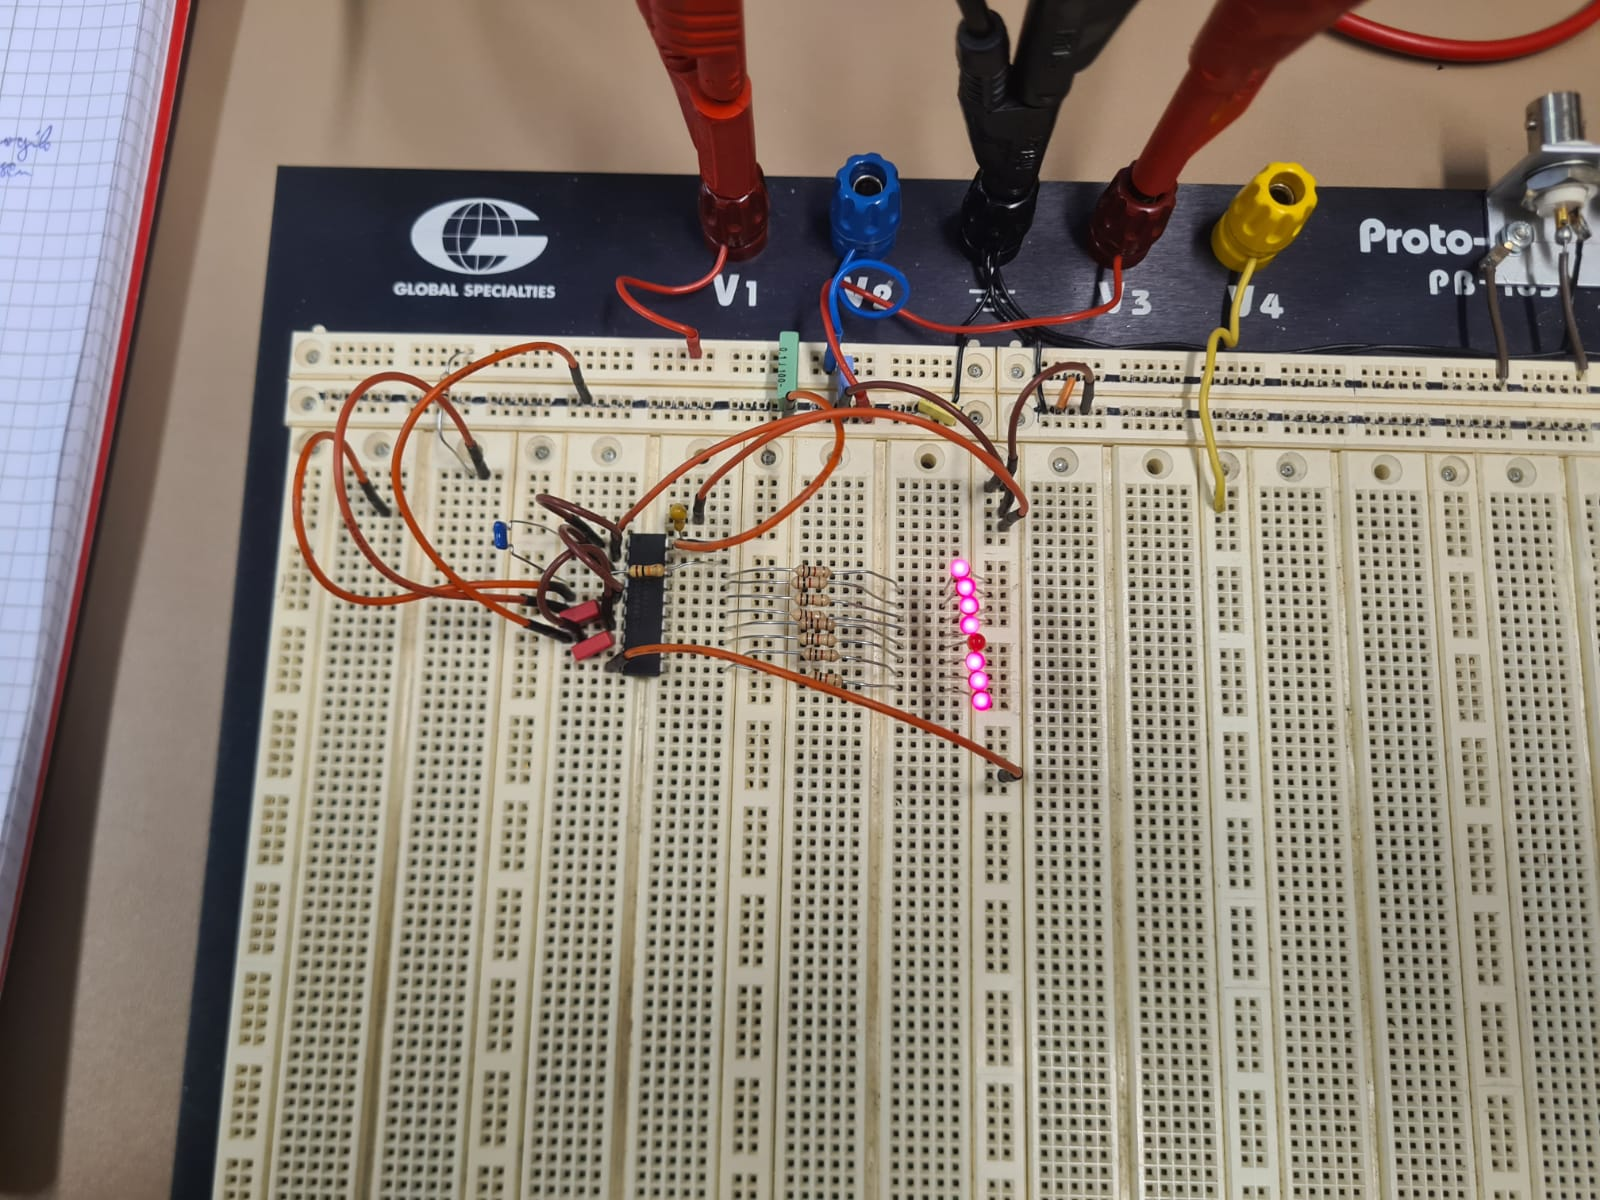
\includegraphics[width=0.5\textwidth]{versuch_1_versuchsaufbau.jpeg}
  \caption{Versuchsaufbau}
  \label{abb:aufbau1}
\end{figure}

Dafür wird die Schaltung %TODO schaltskitze einfügen
und der Versuchsaufbau in Abbildung \ref{abb:aufbau1} verwendet. \\
Dabei ist zu beachten, dass der Analoge Masseanschluss und der Digitale Masseanschluss des \ac{adc}
bis zum Netzgerät getrennt verlaufen sollten, um Störungen zu vermeiden.

Die Logik Ausgänge des \ac{adc} sind low-aktive \ac{ttl} Ausgänge.
Dadurch wird ein 1 Bitwert von einer nicht leuchtenden \ac{led} symbolisiert.
Die \ac{led}s können auch nicht umgekehrt beschalten werden, da das zu Störungen im \ac{adc} führen würde.

% \printbibliography

\end{document}